\documentclass[tikz,border=6pt]{standalone}
\usepackage{pgfplots}
\pgfplotsset{compat=1.18}
\definecolor{curveblue}{RGB}{37,99,235}
\definecolor{lineorange}{RGB}{234,88,12}
\definecolor{pointgreen}{RGB}{5,150,105}
\definecolor{axisgray}{RGB}{100,116,139}
\begin{document}
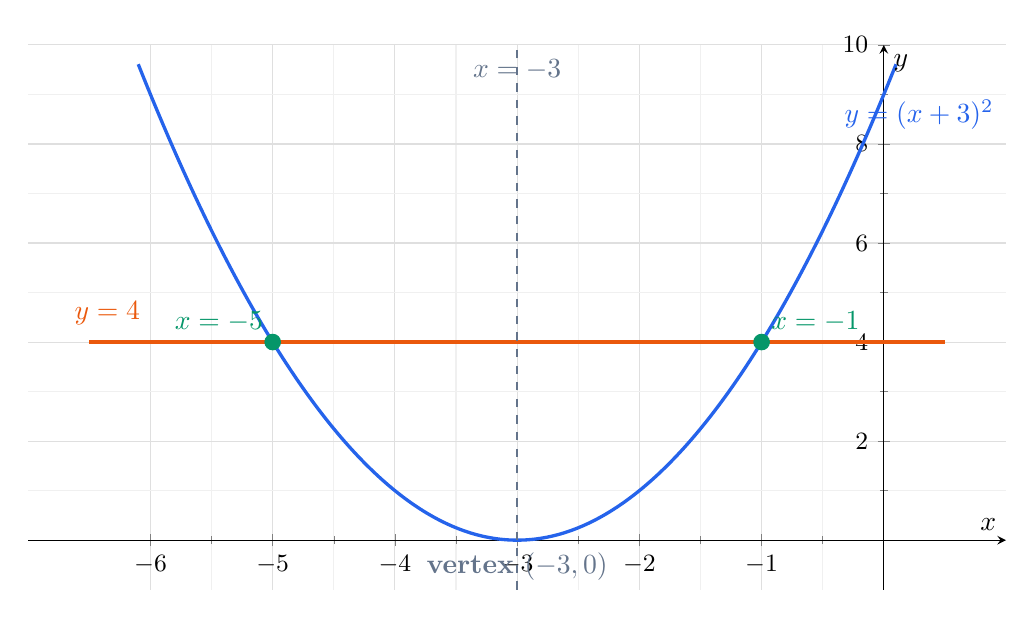
\begin{tikzpicture}
\begin{axis}[
  width=14cm,
  height=8.5cm,
  axis lines=middle,
  xlabel={$x$},
  ylabel={$y$},
  xmin=-7,
  xmax=1,
  ymin=-1,
  ymax=10,
  xtick={-6,-5,-4,-3,-2,-1,0},
  ytick={0,2,4,6,8,10},
  grid=both,
  minor tick num=1,
  major grid style={draw=gray!25},
  minor grid style={draw=gray!12},
  tick label style={font=\small},
  label style={font=\bfseries},
  samples=240,
  clip=false,
]
\addplot[curveblue, very thick, domain=-6.1:0.1] {(x+3)^2};
\addplot[lineorange, very thick, domain=-6.5:0.5] {4};
\addplot[axisgray, dashed, thick] coordinates {(-3,-1) (-3,10)};
\addplot[pointgreen, only marks, mark=*, mark size=2.8pt] coordinates {(-5,4) (-1,4)};
\node[anchor=south west, text=curveblue, font=\bfseries] at (axis cs:-0.4,8.1) {$y=(x+3)^2$};
\node[anchor=south west, text=lineorange, font=\bfseries] at (axis cs:-6.7,4.15) {$y=4$};
\node[anchor=south east, text=pointgreen, font=\bfseries] at (axis cs:-5,4) {$x=-5$};
\node[anchor=south west, text=pointgreen, font=\bfseries] at (axis cs:-1,4) {$x=-1$};
\node[anchor=south, text=axisgray, font=\bfseries] at (axis cs:-3,9.1) {$x=-3$};
\node[anchor=north, text=axisgray, font=\bfseries] at (axis cs:-3,-0.05) {vertex $(-3,0)$};
\end{axis}
\end{tikzpicture}
\end{document}
